\documentclass[11pt,aspectratio=169]{beamer}
\usepackage[utf8]{inputenc} % safe for pdfLaTeX / TexpadTeX
%%%%%%%%% GENERAL PACKAGES
%\usepackage[dvipsnames]{xcolor}
%\usepackage{pdfpages}
%\usetheme[progressbar=frametitle]{metropolis}
%\setbeamercolor{background canvas}{bg=white}
%\usepackage{appendixnumberbeamer}
%\usepackage{booktabs}
%\usepackage[scale=2]{ccicons}
%\usepackage{pgfplots}
%\usepgfplotslibrary{dateplot}
%\usepackage{xspace}
%\newcommand{\themename}{\textbf{\textsc{metropolis}}\xspace}
%\usepackage[absolute,overlay]{textpos}






%%%%%%%%% COLOR THEME

% Define some colors:
\definecolor{DarkFern}{HTML}{407428}
\definecolor{DarkCharcoal}{HTML}{4D4944}
\definecolor{AlertColor}{RGB}{89,124,158}
\definecolor{HighLight}{RGB}{96,95,134}
\definecolor{Important}{RGB}{234,122,133}
\definecolor{Yellow}{HTML}{00539C}
\colorlet{Fern}{DarkFern!85!white}
\colorlet{Charcoal}{DarkCharcoal!85!white}
\colorlet{LightCharcoal}{Charcoal!50!white}
\colorlet{HighLight2}{AlertColor}
\colorlet{DarkRed}{red!70!black}
\colorlet{DarkBlue}{blue!70!black}
\colorlet{DarkGreen}{green!70!black}
\definecolor{RoyalBlue}{HTML}{00539C}
\definecolor{Peach}{HTML}{EEA47F}
\definecolor{ForestGreen}{HTML}{2C5F2D}
\definecolor{MossGreen}{HTML}{E8FCC9}
\definecolor{SeaGreen}{HTML}{2E8B57}
% Use the colors:
\setbeamercolor{title}{fg=Fern}
\setbeamercolor{frametitle}{fg=MossGreen,bg=ForestGreen}
\setbeamercolor{normal text}{fg=Charcoal!70!black}
\setbeamercolor{block title}{fg=black,bg=Fern!25!white}
\setbeamercolor{block body}{fg=black,bg=Fern!10!white}
\setbeamercolor{block title alerted}{fg=black,bg=DarkRed!25!white}
\setbeamercolor{block body alerted}{fg=black,bg=DarkRed!10!white}
\setbeamercolor{alerted text}{fg=DarkRed}
\setbeamercolor{itemize item}{fg=Charcoal}



%%%%%%%%% OTHER COMMANDS
\newcommand{\indep}{\perp\!\!\! \perp}
\newcommand{\comment}[1]{}
\newcommand{\bs}{\boldsymbol}
\newcommand{\tr}{\text{trace}}
\newcommand{\sgn}{{\rm sgn}}
\def\T{\top}
%\newcommand{\det}{\text{det}}
\newcommand{\var}{\mathrm{var}}
\newcommand{\cC}{{\cal C}}
\renewcommand{\d}{{\rm d}}
\newcommand{\cG}{{\cal G}}
\newcommand{\cV}{{\cal V}}
\newcommand{\cE}{{\cal E}}
\newcommand{\cM}{{\cal M}}
\newcommand{\cP}{{\cal P}}
\newcommand{\cX}{{\cal X}}
\newcommand{\cY}{{\cal Y}}
\newcommand{\X}{\mathbf{X}}
\newcommand{\Y}{\mathbf{Y}}
\newcommand{\x}{\mathbf{x}}
\newcommand{\y}{\mathbf{y}}
\newcommand{\z}{\mathbf{z}}

\newcommand{\argmin}{\operatornamewithlimits{argmin}}
\newcommand{\eps}{\varepsilon}
\newcommand{\<}{\langle}
\renewcommand{\>}{\rangle}


%

\setbeamertemplate{navigation symbols}{}
\setbeamertemplate{footline}[text line]{%
    \hfill\strut{%
        \scriptsize\sf\color{black!60}%
        \quad\insertframenumber/\inserttotalframenumber
    }
    %\hfill
    }


\usenavigationsymbolstemplate{}
\setbeamersize{text margin left=.2cm,text margin right=.2cm} 
\addtobeamertemplate{frametitle}{}{\vspace{-1.2mm}}
\setbeamertemplate{itemize item}{$\bullet$}

\setbeamertemplate{itemize subitem}{\tiny\raise1.5pt\hbox{\donotcoloroutermaths$\blacktriangleright$}}
\setbeamertemplate{itemize subsubitem}{\tiny\raise1.5pt\hbox{\donotcoloroutermaths$\blacktriangleright$}}
\setbeamertemplate{enumerate item}{\insertenumlabel.}
\setbeamertemplate{enumerate subitem}{\insertenumlabel.\insertsubenumlabel}
\setbeamertemplate{enumerate subsubitem}{\insertenumlabel.\insertsubenumlabel.\insertsubsubenumlabel}
\setbeamertemplate{enumerate mini template}{\insertenumlabel}






\newcommand{\TODO}[1]{{\color{red}{[TODO: #1]}}}


\newcommand{\R}{\mathbb R}
\newcommand{\E}{\mathbb E}
\renewcommand{\P}{\mathbb P}


\DeclareMathOperator*{\cov}{cov}


\newsavebox{\zerobox}
\newenvironment{nospace}
{\par\edef\theprevdepth{\the\prevdepth}\nointerlineskip
  \setbox\zerobox=\vtop to 0pt\bgroup
  \hrule height0pt\kern\dimexpr\baselineskip-\topskip\relax
}
{\par\vss\egroup\ht\zerobox=0pt \wd\zerobox=0pt \dp\zerobox=0pt
  \box\zerobox}

\usepackage{soul}
\makeatletter
\let\HL\hl
\renewcommand\hl{%
  \let\set@color\beamerorig@set@color
  \let\reset@color\beamerorig@reset@color
  \HL}
  \makeatother


% Title block: keep moving arguments simple (no \\[...])
\title[Calculus and Linear Algebra]{Lecture 4: Calculus and Linear Algebra}
\author[Piotr Zwiernik]{Piotr Zwiernik\\Mathematics Brush-up}
\institute[Barcelona School of Economics]{Barcelona School of Economics}
\titlegraphic{\vspace{-0.5em}
\includegraphics[width=1.5in]{img/bse.png}}
\date{}

\begin{document}

% ------------------------------------------------
\begin{frame}
  \titlepage
\end{frame}
% ------------------------------------------------

% ------------------------------------------------
\begin{frame}{Chapter 9: Functions of several variables}

\begin{Large}
Many economic and data science models depend on \textcolor{SeaGreen}{several variables simultaneously}.
\end{Large}

\vskip 10pt
\textcolor{SeaGreen}{Examples:}
\begin{itemize}
\item \textbf{Economics:} Cobb--Douglas production $Y=K^\alpha L^{1-\alpha}$, or utility $U(x,y)$.
\item \textbf{Data science:} Loss functions $L(\theta_1,\ldots,\theta_d)$ depending on many parameters.
\end{itemize}

\vskip 8pt
\textcolor{SeaGreen}{Reading:} Werner--Sotskov (Ch. 11); Simon--Blume (Chs. 14, 17).\\
\textcolor{SeaGreen}{Exercises:} 11.11(a), 11.21, 11.22 (Werner--Sotskov).
\end{frame}

% ------------------------------------------------
\begin{frame}{What is a multivariable function?}

A \textcolor{SeaGreen}{function of $n$ variables} is a map
\[
f:\ D \subset \R^n \to \R, 
\qquad \mathbf{x}=(x_1,\dots,x_n)\mapsto f(\mathbf{x}).
\]

\begin{itemize}
\item For $n=2$: graph $z=f(x,y)$ is a \textcolor{SeaGreen}{surface} in $\R^3$.
\item \textcolor{SeaGreen}{Level curves} (contours): 
\[
\{(x,y)\in D:\ f(x,y)=c\}.
\]
\item For $n>2$: use \textcolor{SeaGreen}{slices or projections} to visualize.
\end{itemize}
\end{frame}

% ------------------------------------------------
\begin{frame}{Example: quadratic function}

\[
f(x,y)=100-x^2-y^2
\]

\begin{columns}
\column{0.5\textwidth}
\begin{itemize}
\item Graph of $f$: paraboloid.
\item Level curves: concentric circles.
\end{itemize}

\column{0.5\textwidth}
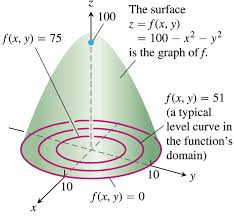
\includegraphics[width=\textwidth]{img/level_curve}
\end{columns}
\end{frame}
% ------------------------------------------------
\begin{frame}{Economic example: Cobb--Douglas}

\textcolor{SeaGreen}{Cobb--Douglas production function}
\[
P(L,K)=b\,L^{\alpha}K^{\beta}.
\]
{\footnotesize
\(P\) = output, \(L\) = labour, \(K\) = capital, \(b\) = total factor productivity, \(\alpha,\beta\) = output elasticities.}
\vskip 6pt
Domain:
\[
D=\{(L,K)\in\R^2:\ L\ge 0,\ K\ge 0\}.
\]

\begin{figure}
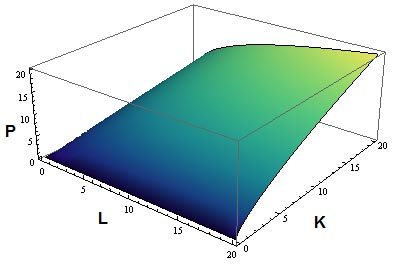
\includegraphics[width=2.5in]{img/cd.jpg}
\end{figure}
\end{frame}

% ------------------------------------------------
\begin{frame}{Returns to scale in Cobb--Douglas}

\begin{itemize}
\item \(\alpha\) (resp.\ \(\beta\)) measures the \textcolor{SeaGreen}{\% change in output} after a \(1\%\) change in labour (resp.\ capital), ceteris paribus.
\item If \(\alpha+\beta=1\), there are \textcolor{SeaGreen}{constant returns to scale}: scaling \((L,K)\) by \(t>0\) scales \(P\) by \(t\).
\item If \(\alpha+\beta<1\), \textcolor{SeaGreen}{decreasing returns}; if \(\alpha+\beta>1\), \textcolor{SeaGreen}{increasing returns}.
\end{itemize}

\end{frame}

% ------------------------------------------------
\begin{frame}{Multivariate Gaussian density}

A random vector \({\bf X}\in\R^d\) is \textcolor{SeaGreen}{multivariate normal} with mean \({\bf m}\) and positive definite covariance \(\Sigma\) if
\[
f({\bf x})=(2\pi)^{-d/2}(\det \Sigma)^{-1/2}
\exp\!\left(-\tfrac12({\bf x}-{\bf m})^{\top}\Sigma^{-1}({\bf x}-{\bf m})\right),
\]
where 
\begin{itemize}
	\item \({\bf m}=E({\bf X})\) is the mean,
	\item \(\Sigma=E\!\big(({\bf X}-{\bf m})({\bf X}-{\bf m})^{\top}\big)\) is the covariance matrix.\\[4mm]
\end{itemize}
Note: $f$ is strictly positive. It depends on $\x$ through the Mahalonobis distance $$\|\x-\bs m\|_{\Sigma}\;:=\;\sqrt{({\bf x}-{\bf m})^{\top}\Sigma^{-1}({\bf x}-{\bf m})}$$
Thus, the level sets are the elipsoids $\{\x:\|\x-\bs m\|={\rm const}\}$.
\end{frame}

% ------------------------------------------------
\begin{frame}{Multivariate Gaussian density}

\textcolor{SeaGreen}{Example:} \(d=2\), \({\bf m}={\bf 0}\), variances \(\sigma_1^2=1\), \(\sigma_2^2=4\) (zero covariance).

\begin{figure}
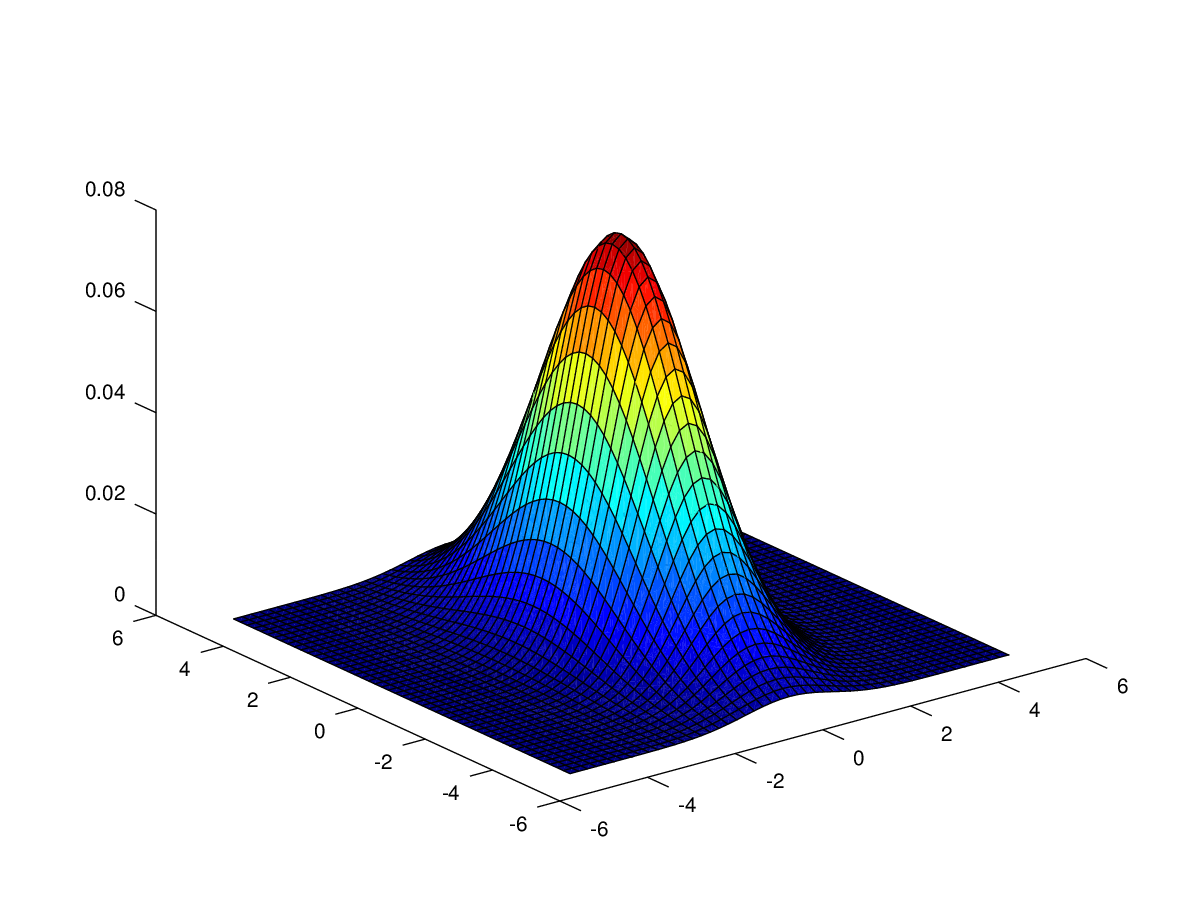
\includegraphics[width=3in]{img/multiv}
\end{figure}
\end{frame}

% ------------------------------------------------
\begin{frame}{Partial derivatives}
\begin{block}{Definition}
For \(f:D\subset\R^2\to\R\), the partial derivatives at \((x,y)\) are
\[
f_x(x,y)=\lim_{h\to 0}\frac{f(x+h,y)-f(x,y)}{h},\qquad
f_y(x,y)=\lim_{h\to 0}\frac{f(x,y+h)-f(x,y)}{h},
\]
when these limits exist.	 (We also use more standar notation $\frac{\partial f}{\partial x}(x,y)$, $\frac{\partial f}{\partial y}(x,y)$)
\end{block}
\begin{alertblock}{}
	Equivalently, fix $y$ and define $g(x)=f(x,y)$. Then $f_x(x,y)=g'(x)$.
\end{alertblock}

\textcolor{SeaGreen}{Example (marginal costs):} if
\[
C(x,y)=200+22x+16y^{3/2},
\]
then \(C_x(x,y)=22\) and \(C_y(x,y)=24\sqrt{y}\).

\end{frame}

% ------------------------------------------------
\begin{frame}{Cobb--Douglas: marginal productivities}

For \(P(L,K)=b\,L^{\alpha}K^{\beta}\),
\[
\frac{\partial P}{\partial L}=\alpha\,\frac{P}{L},\qquad
\frac{\partial P}{\partial K}=\beta\,\frac{P}{K}.
\]
\textcolor{SeaGreen}{Interpretation:} marginal productivity of labour/capital is proportional to average productivity per unit.
{\footnotesize Under suitable regularity, these proportionality laws lead back to the Cobb--Douglas form.}

\end{frame}

\begin{frame}{Tangent plane and linear approximation}

Geometrically, \(f_x(x_0,y_0)\) (resp.\ \(f_y(x_0,y_0)\)) is the slope of the tangent to the curve cut by the plane \(y=y_0\) (resp.\ \(x=x_0\)) at \((x_0,y_0,z_0)\), where \(z_0=f(x_0,y_0)\).

\vskip 6pt
The \textcolor{SeaGreen}{tangent plane} at \((x_0,y_0,z_0)\) is
\[
z = f(x_0,y_0)+f_x(x_0,y_0)(x-x_0)+f_y(x_0,y_0)(y-y_0).
\]

\vskip 6pt
\textcolor{SeaGreen}{Linear (first-order) approximation} near \((x_0,y_0)\):
\[
f(x,y)\approx f(x_0,y_0)+f_x(x_0,y_0)\,\Delta x+f_y(x_0,y_0)\,\Delta y,
\]
\medskip

In differential notation: \(df\approx f_x\,dx+f_y\,dy\).
\end{frame}
% ------------------------------------------------
\begin{frame}{Tangent plane (visual)}
\begin{figure}
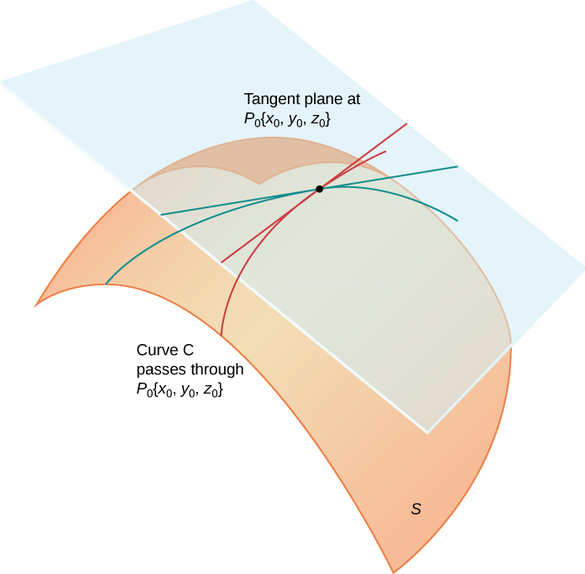
\includegraphics[width=3in]{img/tp.jpg}
\end{figure}
\end{frame}

% ------------------------------------------------
\begin{frame}{Higher partial derivatives}

Higher derivatives are defined by iterating partials, e.g.
\[
f_{xy}(x,y)=\frac{\partial}{\partial y}\!\left(\frac{\partial f}{\partial x}(x,y)\right)
=\frac{\partial^2 f}{\partial y\,\partial x}(x,y).
\]
\vskip 6pt
\textcolor{SeaGreen}{Young's theorem:} If \(f_{xy}\) and \(f_{yx}\) are continuous near a point, then \(f_{xy}=f_{yx}\) there.
\vskip 4pt
\textcolor{SeaGreen}{Example:} \(f(x,y)=\sin(3x-y)\Rightarrow f_{xy}=f_{yx}=3\sin(3x-y)\).

\end{frame}

% ------------------------------------------------
\begin{frame}[label=LinAp]{The gradient and linear approximation}

For ${\bf x}\in\R^n$, the \textcolor{SeaGreen}{gradient} is
\[
\nabla f({\bf x})=\big(f_{x_1}({\bf x}),\dots,f_{x_n}({\bf x})\big).
\]

\vskip 6pt
\begin{alertblock}{best linear approximation}	
If $f$ is a $C^1$-function, then for $\bs h\in \R^n$,
\[
f({\bf x}+\bs h)=f({\bf x})+\langle \nabla f({\bf x}),\bs h\rangle + o(\|\bs h\|).
\]

So the gradient gives the \alert{best linear approximation} of $f$ near ${\bf x}$.
\end{alertblock}
\end{frame}

% ------------------------------------------------
\begin{frame}{Why is the gradient the direction of steepest ascent?}

Take $\bs h=t\bs u$ with $\|\bs u\|=1$, $t>0$ small. Then
\[
f({\bf x}+t\bs u) = f({\bf x}) + t\,\langle \nabla f({\bf x}),\bs u\rangle+o(t).
\]

\vskip 6pt
The instantaneous rate of change in direction $\bs u$ is
\[
D_u f({\bf x})\;:=\;\lim_{t\to 0}\frac{f({\bf x}+t\bs u)-f({\bf x})}{t} \;=\; \langle \nabla f({\bf x}),u\rangle.
\]

\vskip 6pt
By Cauchy–Schwarz,
\[
|D_u f({\bf x})| \le \|\nabla f({\bf x})\|,
\]
with equality if $u$ points in the same direction as $\nabla f({\bf x})$.

\vskip 6pt
\textcolor{SeaGreen}{Conclusion:}  
$\nabla f({\bf x})$ points in the direction of \alert{steepest increase},  
$-\nabla f({\bf x})$ in the direction of \alert{steepest decrease}.
\end{frame}

% ------------------------------------------------
\begin{frame}{Example: gradient and level curves}
\begin{minipage}{6cm}
	\begin{figure}
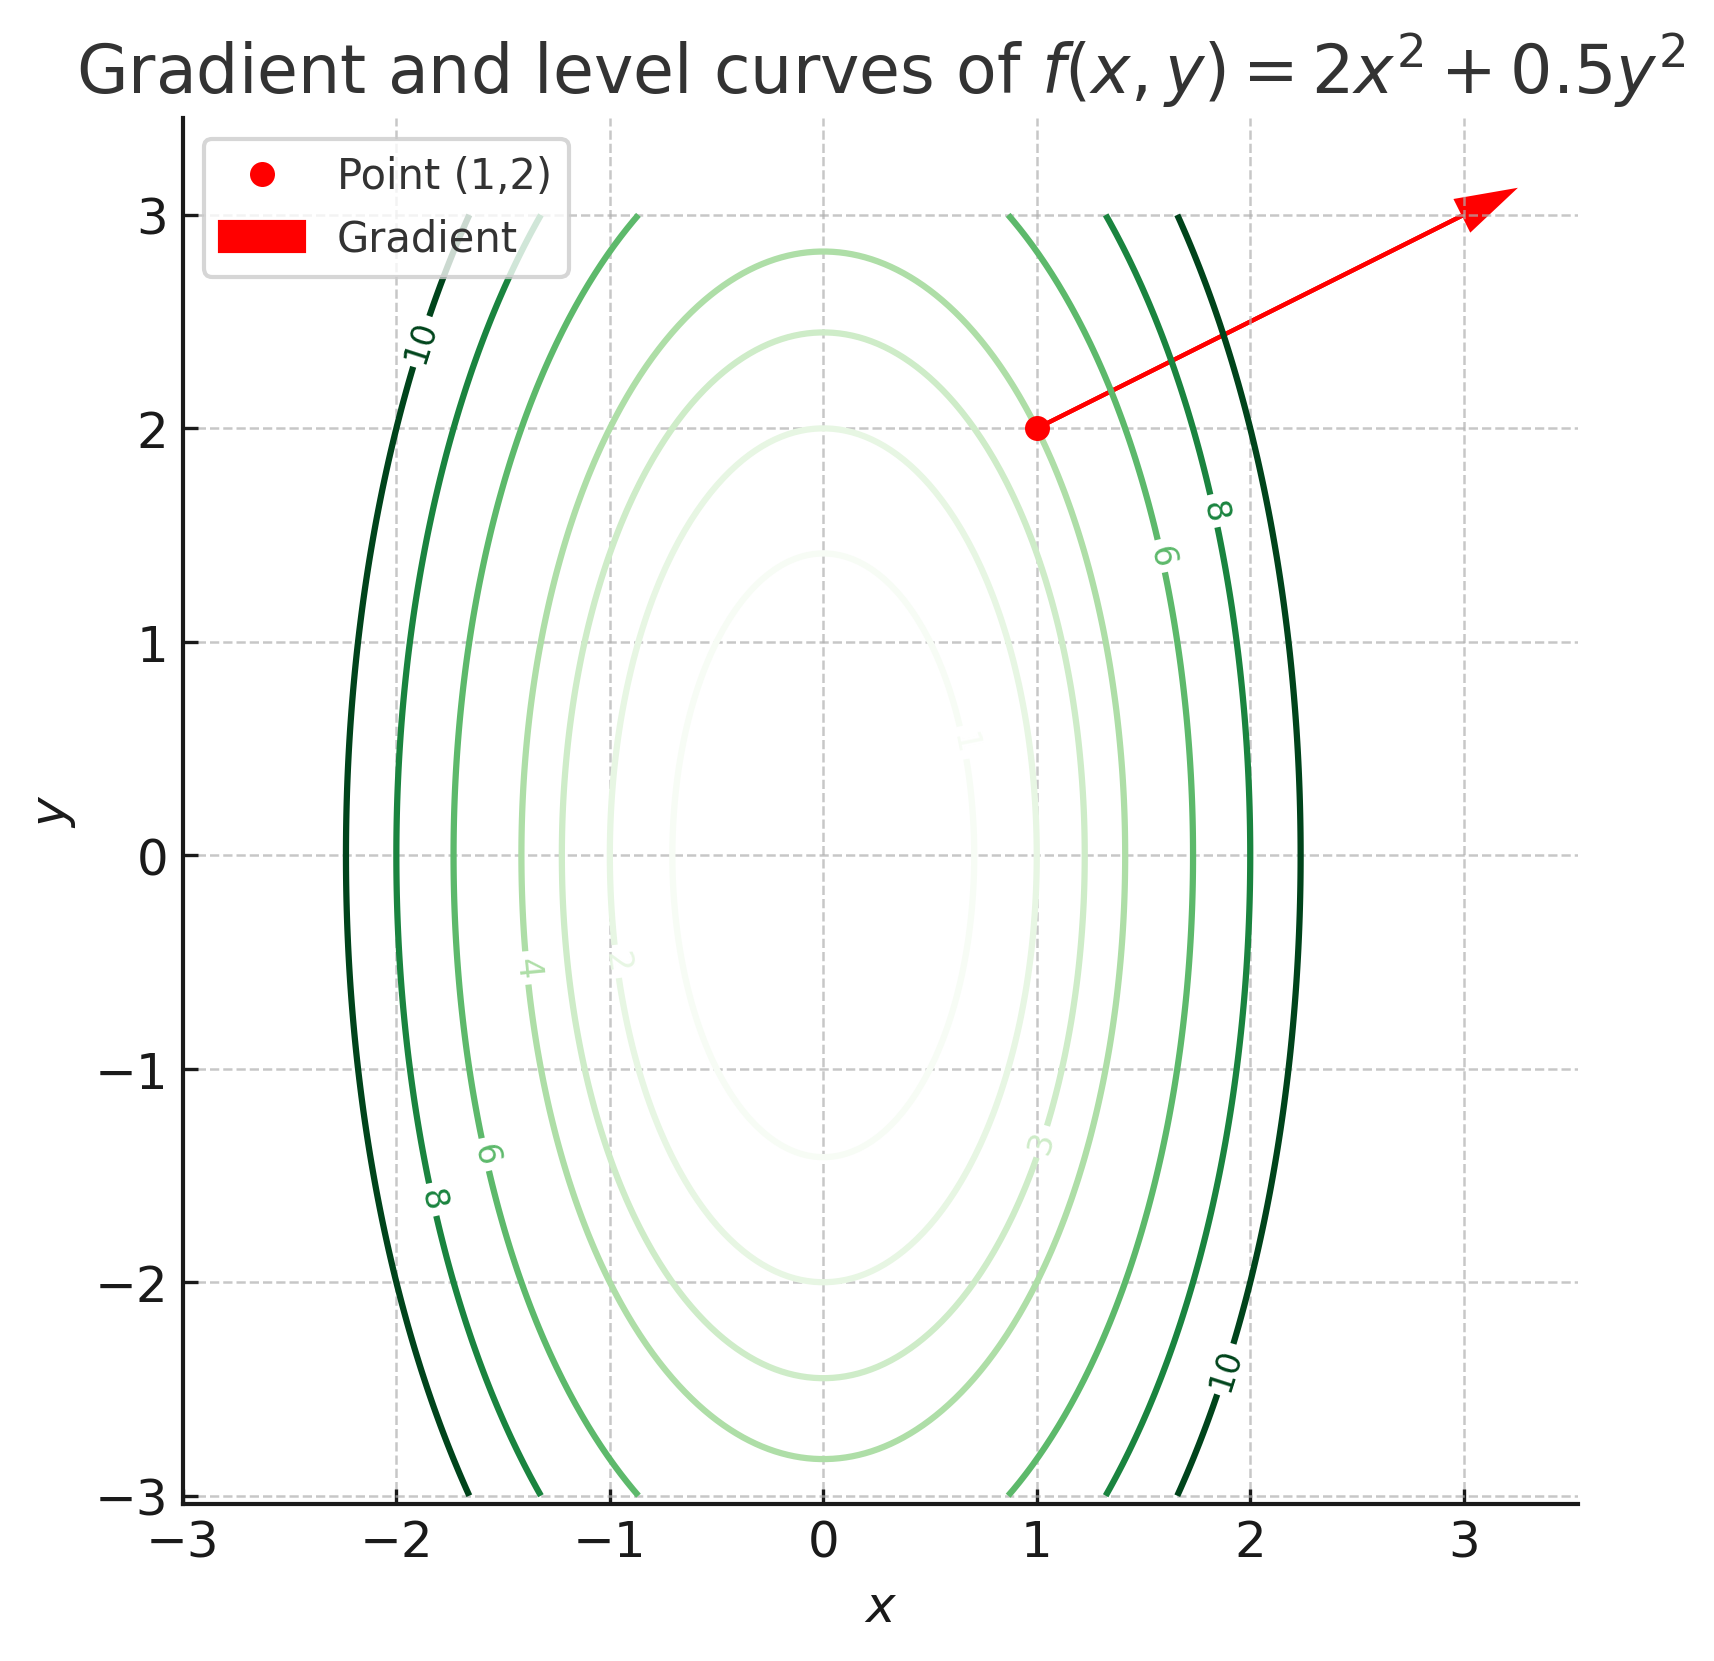
\includegraphics[width=0.95\textwidth]{img/gradient_level_sets}
\end{figure}
\end{minipage}\begin{minipage}{9cm}
	Let $f(x,y)=2x^2+\tfrac12 y^2$.
\[
\nabla f(x,y) = (4x,y).
\]
At $(1,2)$, $\nabla f=(4,2)$.

\vskip 6pt
\textcolor{SeaGreen}{Geometry:}  
The gradient is perpendicular to the level curve 
\[
2x^2+\tfrac12 y^2=c
\]
through $(1,2)$.
\end{minipage}
Note: {$\nabla f$ is always normal to level sets. Why?}

\end{frame}

% ------------------------------------------------
\begin{frame}{Jacobian and matrix differentiation rules}

Let \(F:\R^n \to \R^m\).  
The \textcolor{SeaGreen}{Jacobian matrix} of \(F\) at \({\bf x}\in\R^n\) is
\[
{\rm J}F({\bf x}) = 
\left[\frac{\partial F_i}{\partial x_j}({\bf x})\right]_{i=1,\dots,m;\,j=1,\dots,n}
\in \R^{m\times n}.
\]

\begin{itemize}
\item If \(m=1\), then \(F=f:\R^n \to \R\) and  
\({\rm J}f({\bf x}) = \nabla f({\bf x})^{\top}\).
\end{itemize}

\vskip 8pt
\textcolor{SeaGreen}{Useful identities:}
\begin{enumerate}
\item If \(F({\bf x})=A{\bf x}\) with \(A\in\R^{m\times n}\), then \({\rm J}F({\bf x}) = A\).
\item If \(f({\bf x})={\bf a}^{\top}{\bf x}\) with \({\bf a}\in\R^n\), then \(\nabla f({\bf x})={\bf a}\).
\item If \(f({\bf x})={\bf x}^{\top}A{\bf x}\) with \(A\in\R^{n\times n}\), then  
\(\nabla f({\bf x})=(A+A^{\top}){\bf x}\).  
If \(A\) is symmetric: \(\nabla f({\bf x})=2A{\bf x}\).
\end{enumerate}

\end{frame}
% ------------------------------------------------
\begin{frame}{Unconstrained optimization}

A point \({\bf x}_0\) is a \textcolor{SeaGreen}{local maximum} (\textcolor{SeaGreen}{minimum}) if there exists a ball \(B_r({\bf x}_0)\subset D\) such that
\[
f({\bf x})\le f({\bf x}_0)\quad (\text{resp.\ } f({\bf x})\ge f({\bf x}_0))
\quad\text{for all }{\bf x}\in B_r({\bf x}_0).
\]
If this holds on all of \(D\), the optimum is \textcolor{SeaGreen}{global}.
\vskip 6pt
If \({\bf x}_0\) is an interior local extremum and \(f\) is differentiable, then the \textcolor{SeaGreen}{first-order condition} holds:
\[
\nabla f({\bf x}_0)={\bf 0}.
\]
Such points are \textcolor{SeaGreen}{stationary}; a stationary point that is neither max nor min is a \textcolor{SeaGreen}{saddle}.\\[4mm]

Indeed: By Slide~\ref{LinAp}, if $\nabla f({\bf x}_0)\neq {\bf 0}$, an infinitesimal move can increase/decrease the value of $f$.
\end{frame}

% ------------------------------------------------
\begin{frame}{Unconstrained optimization (pictures)}
\begin{figure}
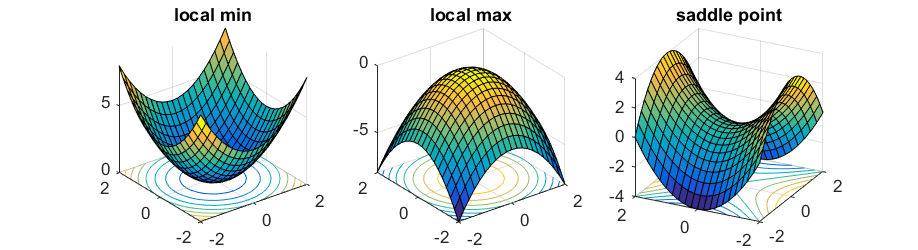
\includegraphics[width=5in]{img/minmaxsaddle.png}
\end{figure}
\end{frame}

% ------------------------------------------------
\begin{frame}{Local optimality: second-order tests}

Assume \(f\in C^2\) and let \(H_f({\bf x})=[f_{x_i x_j}({\bf x})]_{i,j}\) be the (symmetric) Hessian.
\vskip 6pt
\textcolor{SeaGreen}{At a stationary point \({\bf x}_0\):}
\begin{itemize}
\item \(H_f({\bf x}_0)\) positive definite \(\Rightarrow\) local minimum.
\item \(H_f({\bf x}_0)\) negative definite \(\Rightarrow\) local maximum.
\item \(H_f({\bf x}_0)\) indefinite \(\Rightarrow\) saddle.
\end{itemize}
\vskip 6pt
\textcolor{SeaGreen}{\(n=2\) test:} Let \(D_2=f_{xx}f_{yy}-f_{xy}^2\) at \({\bf x}_0\).
\[
\begin{array}{l}
D_2>0,\ f_{xx}>0 \Rightarrow \text{local min},\\
D_2>0,\ f_{xx}<0 \Rightarrow \text{local max},\\
D_2<0 \Rightarrow \text{saddle},\quad D_2=0:\ \text{inconclusive}.
\end{array}
\]

\end{frame}

% ------------------------------------------------
\begin{frame}{Examples}

\begin{enumerate}
\item \(f(x,y)=x^2-y^2-xy\). Then \(\nabla f=(2x-y,\,-2y-x)\). The only stationary point is \((0,0)\). The Hessian
\(
H_f=\begin{pmatrix}2&-1\\ -1&-2\end{pmatrix}
\)
is \textcolor{SeaGreen}{indefinite} \(\Rightarrow\) \((0,0)\) is a \textcolor{SeaGreen}{saddle}.
\item \(f(x,y)=x^2+y^4\). Stationary point: \((0,0)\). 
\(
H_f(0,0)=\begin{pmatrix}2&0\\ 0&0\end{pmatrix}
\)
is positive semidefinite; \(f\ge 0\) so \((0,0)\) is a \textcolor{SeaGreen}{global minimum}.
\item \(f(x,y)=x^3+y^3\). Stationary point: \((0,0)\). The Hessian at \((0,0)\) is \(0\); the point is a \textcolor{SeaGreen}{saddle}.
\end{enumerate}

\end{frame}

% ------------------------------------------------
\begin{frame}{Convex domains}

A set \(D\subset\R^n\) is \textcolor{SeaGreen}{convex} if for any \({\bf x},{\bf y}\in D\) and \(t\in[0,1]\), the point \((1-t){\bf x}+t{\bf y}\in D\).

\begin{figure}
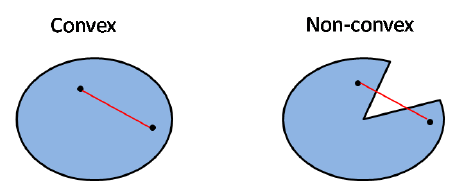
\includegraphics[width=4in]{img/convex_set}
\end{figure}
\end{frame}

% ------------------------------------------------
\begin{frame}{Convexity, concavity, and global optimality}

\begin{alertblock}{Definition (Convexity/Concavity)}
Let \(D \subset \R^n\) be convex.  
A function \(f:D\to\R\) is \textcolor{SeaGreen}{convex} if for all \({\bf x},{\bf y}\in D\) and \(\theta\in[0,1]\),
\[
f(\theta{\bf x}+(1-\theta){\bf y}) 
\;\leq\; \theta f({\bf x})+(1-\theta)f({\bf y}),
\]
i.e.\ the graph lies \emph{below} every chord.\\[2mm]
$\bullet$  $f$ is \textcolor{SeaGreen}{concave} if the inequality is reversed,
i.e.\ the graph lies \emph{above} every chord.
\end{alertblock}

\medskip
\begin{block}{Curvature test (for \(C^2\) functions)}
\begin{enumerate}
\item \(H_f({\bf x})\succeq 0\) on \(D\) \(\;\Leftrightarrow\;\) \(f\) convex.  
      \(H_f({\bf x})\preceq 0\) on \(D\) \(\;\Leftrightarrow\;\) \(f\) concave.
\item Strict definiteness implies strict convexity/concavity.
\end{enumerate}
\end{block}

\medskip
\textcolor{SeaGreen}{Key fact:} If \(f\) is convex (concave) on \(D\), any stationary point is a \textbf{global} minimum (maximum).

\end{frame}

% ------------------------------------------------
\begin{frame}{Example}

Let \(f(x,y)=2x-y-x^2+xy-y^2\). Then
\[
\nabla f=(2-2x+y,\ -1+x-2y),\qquad
H_f=\begin{pmatrix}-2&1\\[2pt]1&-2\end{pmatrix}.
\]
\(H_f\) is \textcolor{SeaGreen}{negative definite} \(\Rightarrow\) \(f\) is strictly concave. The unique stationary point solves \(\nabla f={\bf 0}\), giving \((x,y)=(0,1)\), which is a \textcolor{SeaGreen}{global maximum}.

\begin{figure}
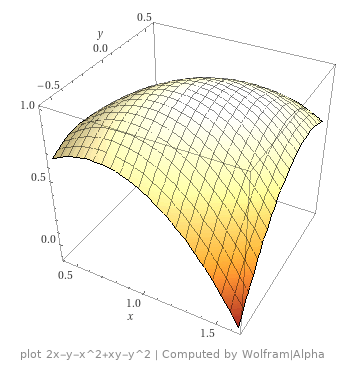
\includegraphics[width=2in]{img/plotxy}
\end{figure}
\end{frame}

% ------------------------------------------------
\begin{frame}{Economic example: profit maximization}

A firm sells products \(X/Y\) at \(45/55\) euros. Revenue \(R(x,y)=45x+55y\). Cost
\[
C(x,y)=300+x^2+1.5\,y^2-25x-35y.
\]
Profit \(f(x,y)=R(x,y)-C(x,y)\). Then
\[
f_x=-2x+70,\qquad f_y=-3y+90 \ \Rightarrow\ (x^\ast,y^\ast)=(35,30).
\]
Since \(H_f=\begin{pmatrix}-2&0\\[2pt]0&-3\end{pmatrix}\) is negative definite everywhere, \(f\) is strictly concave and \((35,30)\) is the \textcolor{SeaGreen}{global maximum}. The maximal profit is \(f(35,30)=2275\).

\end{frame}

% ------------------------------------------------
\begin{frame}{Least squares as orthogonal projection}
Given data $X\in\R^{n\times d}$ and response $y\in\R^n$, the least–squares estimator solves
\[
\hat\beta=\arg\min_\beta \|y-X\beta\|^2,
\qquad
\hat y=X\hat\beta.
\]
\textcolor{SeaGreen}{Geometric view (recall Lecture 2):} $\hat y$ is the orthogonal projection of $y$ onto the column space $\mathcal C(X)$, hence
\[
X^\top (y-X\hat\beta)=0
\quad\Longleftrightarrow\quad
(X^\top X)\hat\beta=X^\top y
\ \ (\text{if $X^\top X$ invertible}).
\]

\medskip
\textcolor{SeaGreen}{Polynomial regression:}  
A common use of least squares is fitting nonlinear trends by expanding the design matrix $X$.  
For instance, with one predictor $x$, we can set
\[
X=\begin{pmatrix}
1 & x_1 & x_1^2 & \cdots & x_1^m\\
\vdots & \vdots & \vdots & & \vdots \\
1 & x_n & x_n^2 & \cdots & x_n^m
\end{pmatrix},
\]
so that the fitted model is $y\approx c_0+c_1 x+\cdots+c_m x^m$.
\end{frame}
% ------------------------------------------------
\begin{frame}{Ridge regression: stabilizing high–variance fits}
When $X^\top X$ is ill-conditioned or $d$ is large, add $\ell_2$ regularization:
\[
\hat\beta_\lambda=\arg\min_\beta \big(\|y-X\beta\|^2+\lambda\|\beta\|^2\big)
\quad\Longrightarrow\quad
\hat\beta_\lambda=(X^\top X+\lambda I)^{-1}X^\top y.
\]
\textcolor{SeaGreen}{Spectral view:} if $X^\top X=U{\rm diag}(s_1^2,\ldots,s_d^2)U^\top$, then
\[
\hat\beta_\lambda
=\sum_{j=1}^d \frac{s_j}{s_j^2+\lambda}\, u_j\, \langle y,\, X u_j\rangle,
\]
so ridge \textcolor{SeaGreen}{shrinks} directions with small $s_j$ (low variance) the most $\big(\tfrac{s_j}{s_j^2+\lambda}<\tfrac1{s_j}\big)$, reducing variance and overfitting.
\end{frame}

% ------------------------------------------------
\begin{frame}{Overfitting vs. ridge: degree-9 polynomial demo}
\alert{$n=10$ points} from $y=\sin x+\varepsilon$ on $[-3,3]$, \alert{degree $9$} polynomial.
\[
\text{OLS (no penalty)} \quad \text{vs.}\quad \text{Ridge with }\lambda=\tfrac13.
\]
\begin{figure}
\centering
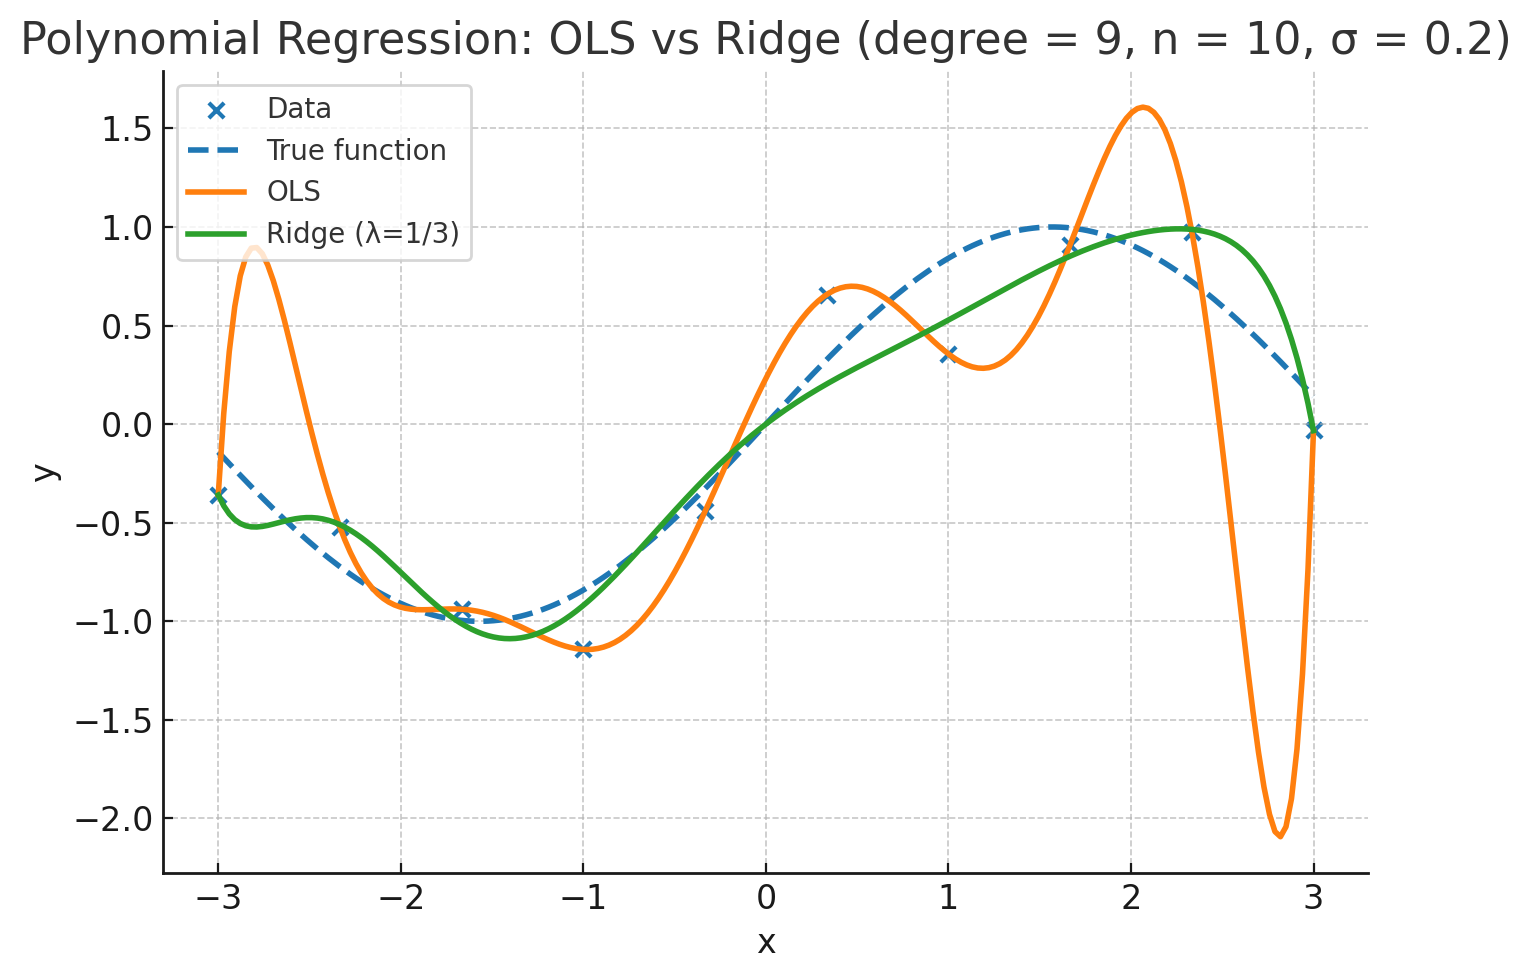
\includegraphics[width=0.6\textwidth]{img/ridge_overfitting.png}
\end{figure}
{\footnotesize OLS wiggles violently between sparse points; ridge damps the high-frequency coefficients and tracks the signal more smoothly.}
\end{frame}


% ------------------------------------------------
\begin{frame}{Modern applied examples (multivariable)}

\begin{itemize}
\item \textcolor{SeaGreen}{Portfolio risk (mean--variance):}
\[
f({\bf w})={\bf w}^{\top}\Sigma\,{\bf w},\quad
g({\bf w})=\mu^{\top}{\bf w},\quad
{\bf w}\in\R^n,\ \sum_i w_i=1,\ w_i\ge 0.
\]
\item \textcolor{SeaGreen}{Logistic regression (binary choice):}
\[
J(\beta)=\frac{1}{n}\sum_{i=1}^n\!\Big(\log\big(1+e^{x_i^{\top}\beta}\big)-y_i\,x_i^{\top}\beta\Big)
\quad(\text{convex in }\beta).
\]
\item \textcolor{SeaGreen}{CES utility/production:}
\[
U(x)=\Big(\sum_{i=1}^n \alpha_i x_i^{\rho}\Big)^{\!1/\rho},\quad
P(L,K)=A\big(\theta\big)\,L^{\alpha}K^{\beta}.
\]
\end{itemize}

\end{frame}


% ------------------------------------------------
\begin{frame}{Gradient descent }

Goal: minimize \(f(\theta)\).
\[
\theta_{t+1}=\theta_t-\eta_t\,\nabla f(\theta_t).
\]
\textbf{Pieces you pick:}
\begin{itemize}
\item \textbf{Step size} \(\eta_t\): constant, diminishing, or via backtracking.
\item \textbf{Stop} when \(\|\nabla f(\theta_t)\|\) small.
%\item \textbf{Guarantee (sketch):} if \(J\) is convex with \(L\)-Lipschitz gradient, then for \(0<\eta<2/L\) constant, GD converges to a global minimizer.
\end{itemize}
{\footnotesize In practice: feature scaling and a good \(\eta_t\) schedule matter a lot.}

\end{frame}

% ------------------------------------------------
\begin{frame}{GD on least squares (closed form vs iterations)}
Least squares problem has a closed form solution. This still requires inverting a potentially large matrix $X^\top X$. GD gives an alternative  way to find a solution. 
\[
f(\beta)=\frac{1}{n}\|X\beta-{\bf y}\|^2,\qquad
\nabla f(\beta)=\frac{2}{n}\,X^{\top}(X\beta-{\bf y}).
\]
\textbf{GD update:}
\[
\beta_{t+1}=\beta_t-\eta\,\frac{2}{n}\,X^{\top}\big(X\beta_t-{\bf y}\big).
\]
\textbf{Ridge:}
\[
f_{\lambda}(\beta)=\frac{1}{n}\|X\beta-{\bf y}\|^2+\lambda\|\beta\|_2^2,\quad
\nabla f_{\lambda}=\frac{2}{n}X^{\top}(X\beta-{\bf y})+2\lambda\beta.
\]
{\footnotesize Closed form exists \((X^{\top}X)^{-1}X^{\top}{\bf y}\), but GD scales better to huge \(n,p\) or streaming data.}

\end{frame}


% ------------------------------------------------
\begin{frame}{Constrained optimization: Lagrange and KKT (teaser)}

Equality constraints \(g_i(x)=0\) and inequality constraints \(h_j(x)\le 0\).
The Lagrangian:
\[
\mathcal{L}(x,\lambda,\mu)=f(x)+\sum_i \lambda_i g_i(x)+\sum_j \mu_j h_j(x).
\]
\textbf{KKT conditions} (when they apply):
\begin{itemize}
\item \textbf{Stationarity: } \(\nabla_x \mathcal{L}(x^*,\lambda^*,\mu^*)=\mathbf{0}\).
\item \textbf{Primal feasibility: } \(g_i(x^*)=0,\; h_j(x^*)\le 0\).
\item \textbf{Dual feasibility: } \(\mu_j^*\ge 0\).
\item \textbf{Complementary slackness: } \(\mu_j^*\,h_j(x^*)=0\).
\end{itemize}
\textbf{Example (budgeted utility max):} maximize \(U(x)\) s.t. \(p^{\top}x\le B\).
Then \(\mathcal{L}(x,\mu)=U(x)+\mu\,(B-p^{\top}x)\) and at optimum
\(\nabla U(x^*)=\mu^* p\), \(p^{\top}x^*\le B\), \(\mu^*\ge 0\), \(\mu^*(B-p^{\top}x^*)=0\).

\end{frame}

% ------------------------------------------------
\begin{frame}{When to use second order methods?}

In general, we update $\theta_t$ as
$$
\theta_{t+1}\;:=\;\arg\min f(\theta_t)+\<\nabla f(\theta_t),\theta\>+\tfrac12 (\theta-\theta_t)^\top \alert{K} (\theta-\theta_t).
$$
If $\alert{K}=I_n$, we recover gradient descent. \\[2mm]
If $\alert{K}=\nabla\nabla^\top f(\theta_t)$, we get the \textcolor{SeaGreen}{Newton method}. \\[2mm]


\begin{itemize}
\item \textbf{Newton:} \(\theta_{t+1}=\theta_t-H^{-1}(\theta_t)\nabla J(\theta_t)\) (fast near solution, expensive to form/solve).
\item \textbf{Quasi-Newton (e.g., BFGS, L\!-\!BFGS):} approximate \(H^{-1}\) from gradients only; great for medium scale convex problems.
\item \textbf{Takeaway:} for huge data/models use (S)GD; for smaller smooth convex problems, quasi-Newton shines.
\end{itemize}

\end{frame}

% ------------------------------------------------
\end{document}